%%% -*- mode:latex; mode:flyspell -*-

%%% Local Variables:
%%% TeX-master: "mu2e-36575"
%%% End:
\section{Tuning the calorimeter timing resolution}

The calorimeter timing simulation has been significantly improved since the Offline version that was freezed to build the SU2020 repository.

The old timing was largely underestimating the calorimeter time resolution. A better parametrization of the photon propagation time inside the crystal and, most significantly, a better implementation of the noise in the simulation now makes the simulation results much closer to the test beam measurements \cite{MU2E_35540_CALO_TIMING}.

The different components of the calorimeter noise during the first period of data taking have been estimated in \cite{MU2E_35519_CALO_NOISE} assuming the Run Plan reported in \cite{MU2E_33731_RUN1_PLAN}. The results are summarized in table \ref{table:calonoise}. They include electronic noise (measured at cosmic rays stand), the Radiation Induce Noise (RIN) and the Dark Current produced by the neutron radiation damage in the SiPMs (assuming to operate them at $-10^o$ C). A safety factor 2 has been used for the neutron induced noise to reflect the uncertainty of the results of neutron radiation damage measurements.

\begin{table}[htbp]
  \begin{center} 
    \begin{tabular}{|c|c|c|c|c|}
      \hline
      Run 1 Time        & FEE noise  & RIN     &  Dark Noise & Total    \\ 
      \hline
      1 batch start     & 200 keV    & 280 keV &  --         & 344 keV  \\
      1 batch end       & 200 keV    & 280 keV &  450 keV    & 566 keV  \\
      2 bacthes end     & 200 keV    & 400 keV &  492 keV    & 634 keV  \\
      \hline
    \end{tabular}
  \end{center}
  \caption{
  \label{table:calonoise}
    Calorimeter noise levels in different moments of Run 1 as estimated in \cite{MU2E_35519_CALO_NOISE}.
  }
  % \vspace{0.5in}
\end{table}

Using the result in the table we assume an average noise of 455 keV for the 1 batch period and 600 keV for the 2 batches period.

A parametrization of the time resolution as function of the noise level and the energy deposited in a crystal obtained using the latest calorimeter simulation software has been presented in \cite{MU2E_36225_CALO_TIME_RES}. The curves corresponding to 455 keV and 600 keV are the lower dashed lines in figures \ref{fig:calorimeter_timing_resolution_1batch} and \ref{fig:calorimeter_timing_resolution_2batch}.

Table \ref{table:calonoise} doesn't include the time jitter of the accelerator signal. This effect should also be included in the tracker timing simulation. For particle identification the only relevant quantity is the relative time between tracker and calorimeter. We decided not to change the tracker timing simulation and to add the accelerator clock jitter all to the cluster time. Preliminary measurements \cite{MU2E_35392_TIME_JITTER} show a time jitter of 172 ps for 2 DTCs in chain and 217 ps for 7 DTCs in chain. We take 200 ps as our best guess.

Being the update of calorimeter software a too big modification for the SU2020 software repository and aiming to include also the effect of the DTCs time jitter we have modified the CaloCrystalHitFromHit module adding an additional time gaussian smearing to reproduce the wanted time resolution.

Figures  \ref{fig:calorimeter_timing_resolution_1batch} and \ref{fig:calorimeter_timing_resolution_2batch} show the output of the pacthed time resolution simulation as function of the energy deposited in the crystal for the two calorimeter disks in case of 1 or 2 proton bacthes. The agreement with the expected analytical function is shown. The deviations at small energies are not relevant because the time resolution simulation in those regions is known to be less reliable.

\begin{figure}[h]
  \hspace{-0.6in}
  \begin{tikzpicture}
    \node[anchor=south west,inner sep=0] at (-1,0.) {
      % \node[shift={(0 cm,0.cm)},inner sep=0,rotate={90}] at (0,0) {}
      \makebox[\textwidth][c] {
        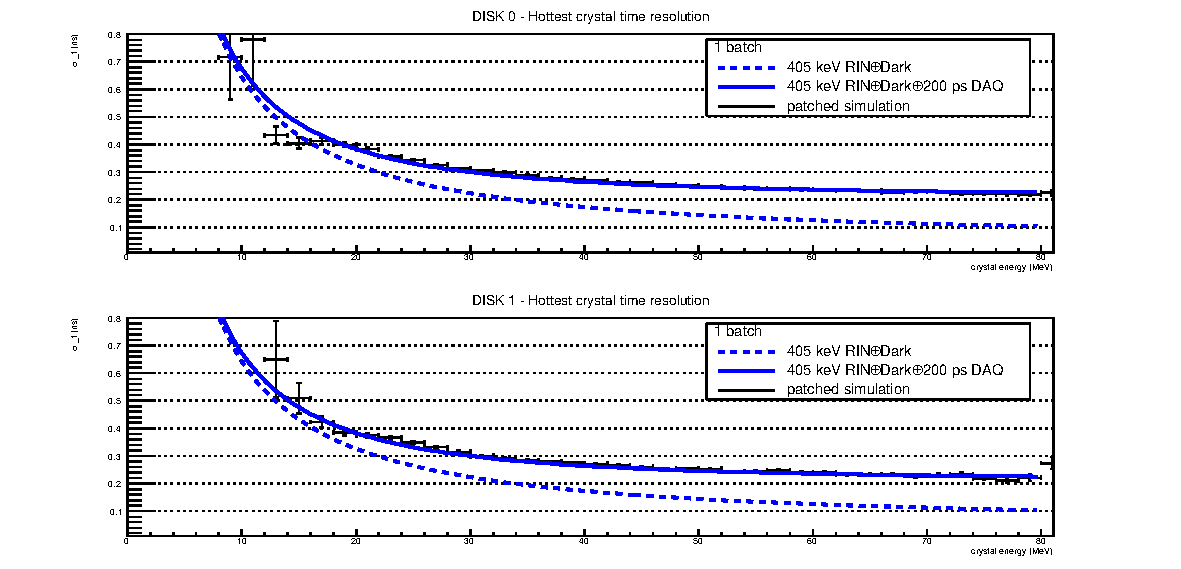
\includegraphics[width=0.80\textwidth]{figures/pdf/figure_00401_sigmat_1batch_corrected}
      }
    };
    % \node [text width=6cm, scale=0.8] at (4.5,6.4) {mu2e-18894 by Kevin Lynch and Jim Popp};
  \end{tikzpicture}
  % \captionof{figure} {
  \caption{
    \label{fig:calorimeter_timing_resolution_1batch}
    Tuning of calorimeter timing resolution for the 1 batch run period. The lower dashed curve corresponds to the parametrization given in \cite{MU2E_36225_CALO_TIME_RES} applying a noise of 455 keV. The upper dashed curve includes the 200 ps for the DTCs time hitter. The black points represent the result of the SU2020 patched calorimeter time simulation.
  }
\end{figure}

\begin{figure}[h]
  \hspace{-0.6in}
  \begin{tikzpicture}
    \node[anchor=south west,inner sep=0] at (-1,0.) {
      % \node[shift={(0 cm,0.cm)},inner sep=0,rotate={90}] at (0,0) {}
      \makebox[\textwidth][c] {
        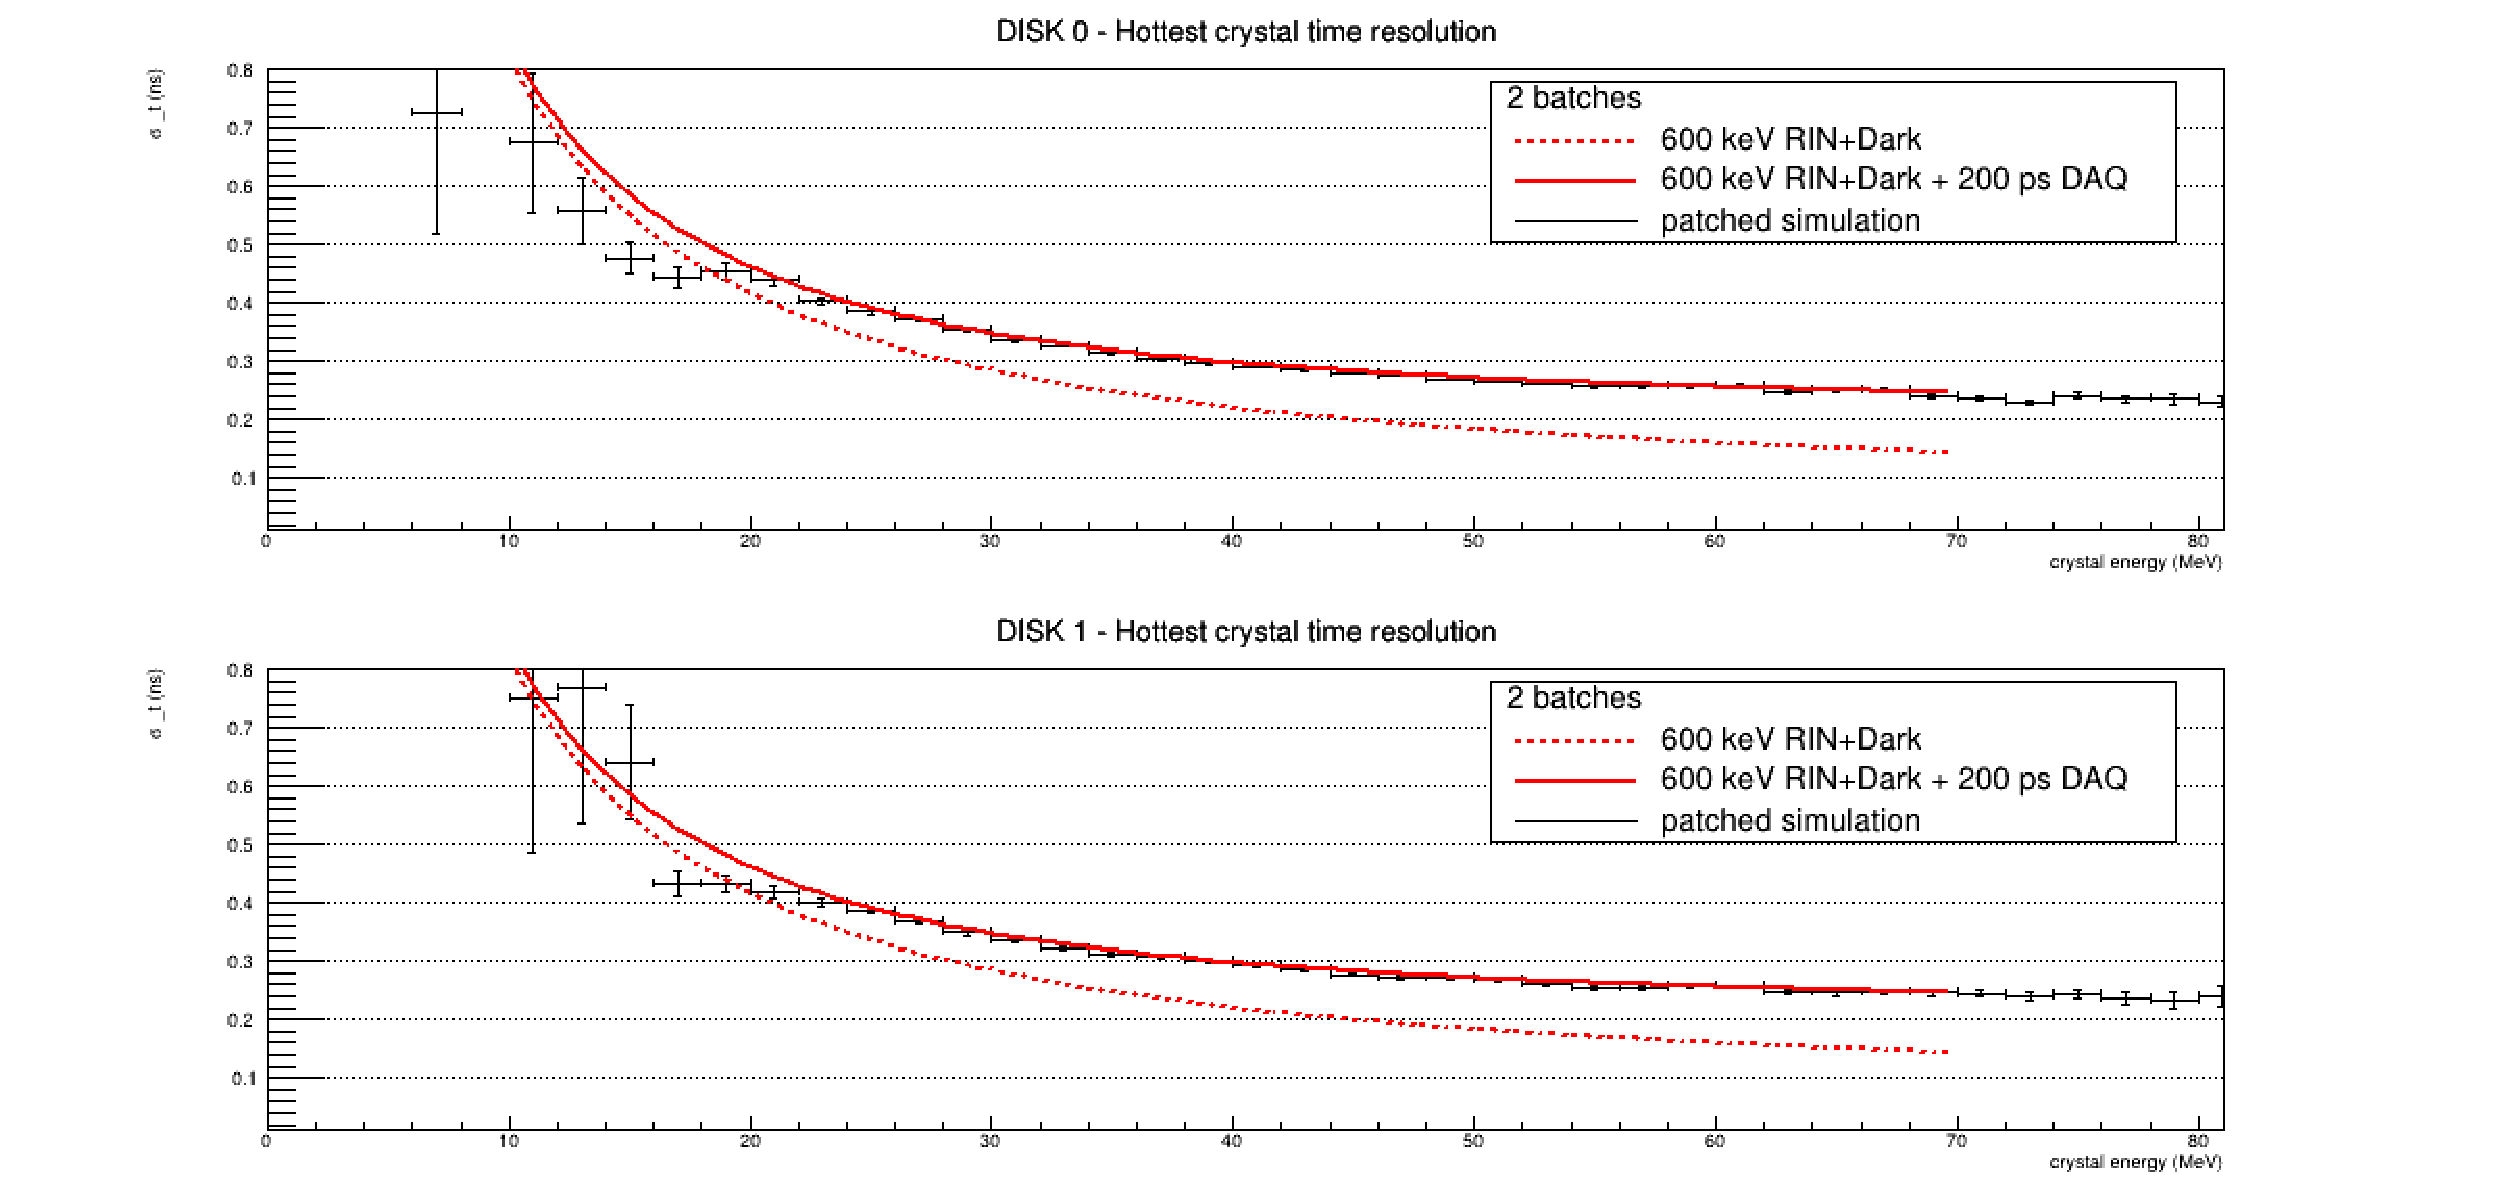
\includegraphics[width=0.80\textwidth]{figures/pdf/figure_00402_sigmat_2batch_corrected}
      }
    };
    % \node [text width=6cm, scale=0.8] at (4.5,6.4) {mu2e-18894 by Kevin Lynch and Jim Popp};
  \end{tikzpicture}
  % \captionof{figure} {
  \caption{
    \label{fig:calorimeter_timing_resolution_2batch}
    Tuning of calorimeter timing resolution for the 2 batches run period. The lower dashed curve corresponds to the parametrization given in \cite{MU2E_36225_CALO_TIME_RES} applying a noise of 600 keV. The upper dashed curve includes the 200 ps for the DTCs time hitter. The black points represent the result of the SU2020 patched calorimeter time simulation. 
  }
\end{figure}
